\section{Appendix}

\subsection{Exercise 5}
\subsubsection{Vocab versus Loss Function Study}
\begin{figure}[H]
    \centering
    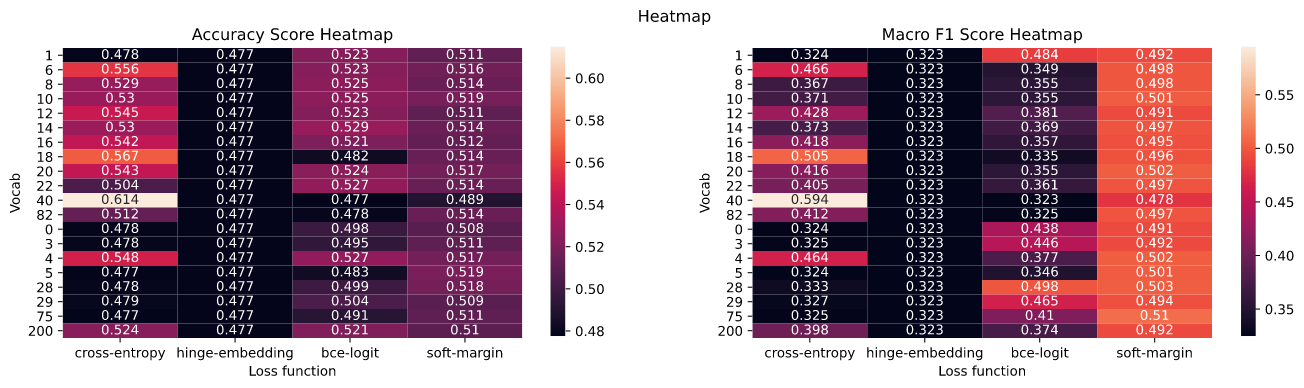
\includegraphics[width=1\linewidth]{pictures/ex5_heatmap_VocabLossFunct.png}
    \caption{Vocab vs Loss Function}
    \label{fig:vocabloss_ex5}
\end{figure}

\subsubsection{Embedding Type Study}
\begin{figure}[H]
    \centering
    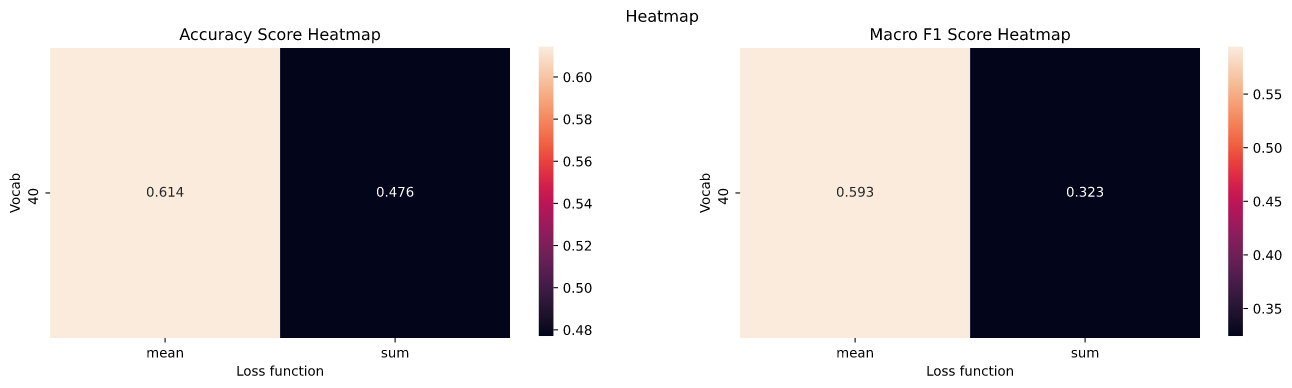
\includegraphics[width=1\linewidth]{pictures/ex5_heatmap_EvdTypeNewVocab.png}
    \caption{Embedding Pool type}
    \label{fig:embtypestudy_ex5}
\end{figure}


\subsubsection{Hidden versus Output Activation Functions Study}
\begin{figure}[H]
    \centering
    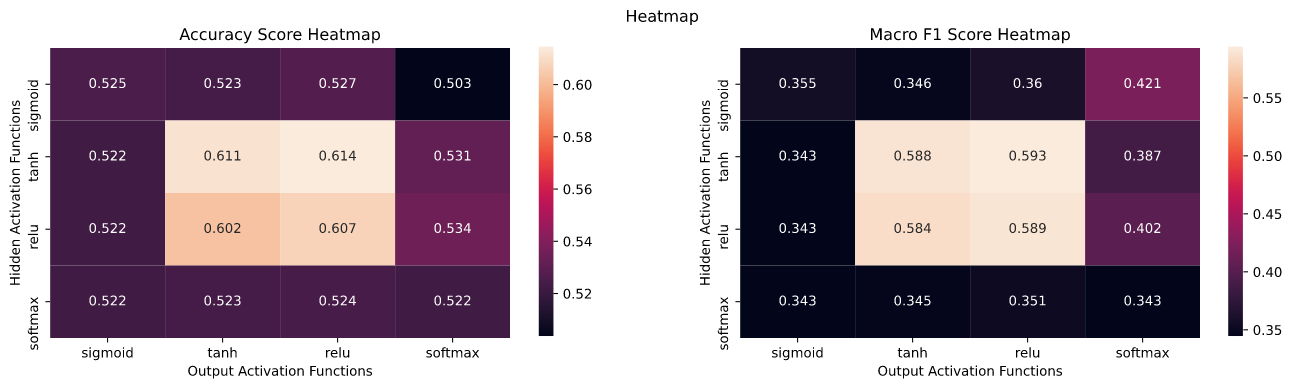
\includegraphics[width=1\linewidth]{pictures/ex5_heatmap_actfunct.png}
    \caption{Activation function study}
    \label{fig:actfunct_ex5}
\end{figure}


\subsubsection{Epochs versus Batch Size Study}
\begin{figure}[H]
    \centering
    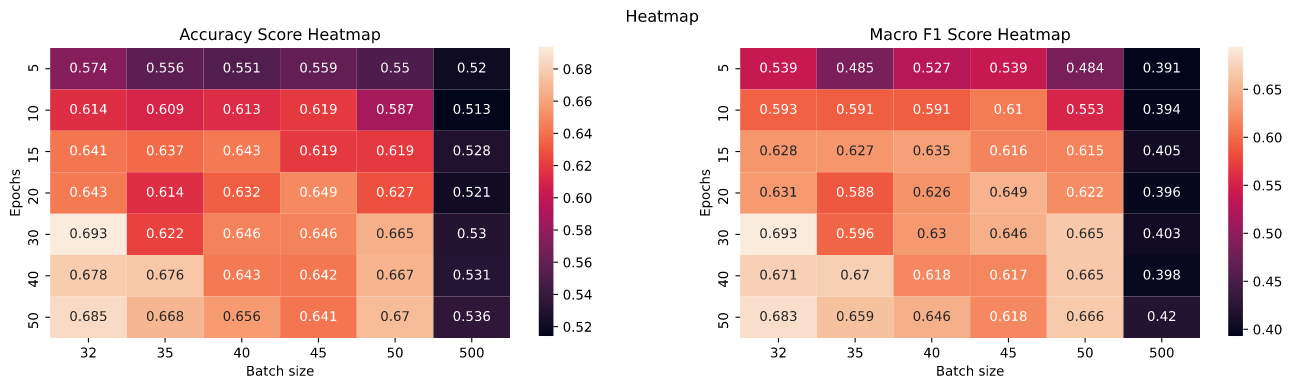
\includegraphics[width=1\linewidth]{pictures/ex5_heatmap_BatchEpoch.png}
    \caption{Epochs vs batch size}
    \label{fig:epochbatch_ex5}
\end{figure}


\subsubsection{Hidden Layers versus Units Study}
\begin{figure}[H]
    \centering
    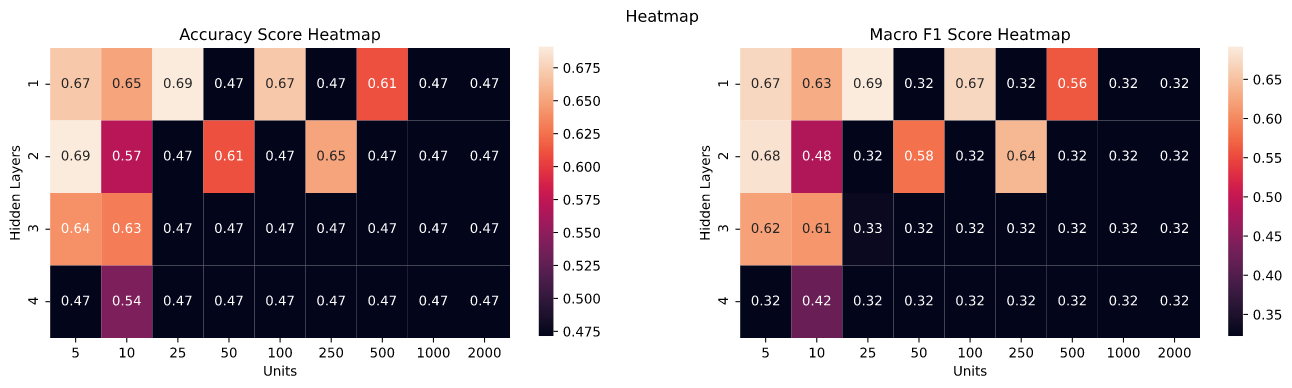
\includegraphics[width=1\linewidth]{pictures/ex5_heatmap_HlUnits.png}
    \caption{Hidden layers vs units per layer}
    \label{fig:hlu_ex5}
\end{figure}

\subsubsection{Learning Rate versus Momentum Study}
\begin{figure}[H]
    \centering
    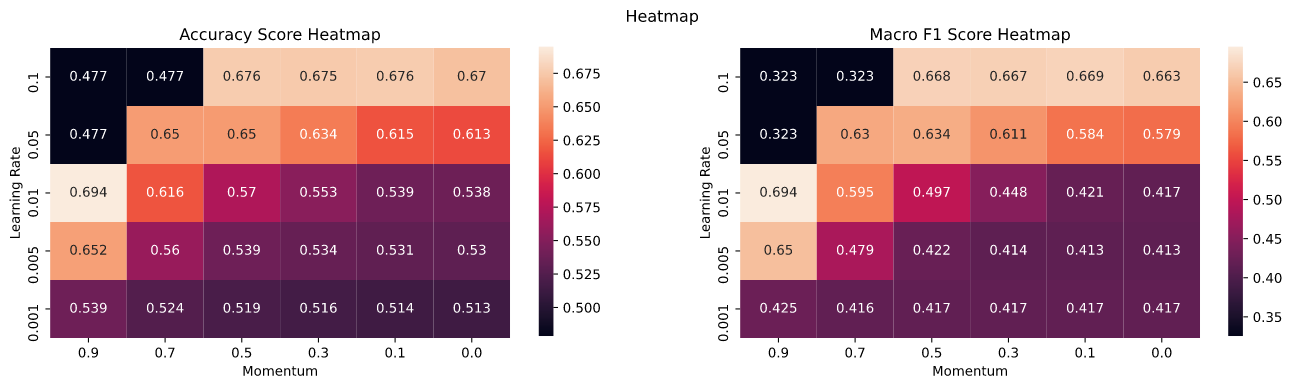
\includegraphics[width=1\linewidth]{pictures/ex5_heatmap_LrMmt.png}
    \caption{Learning rate vs momentum}
    \label{fig:lrmmt_ex5}
\end{figure}
